\documentclass[aspectratio=169,11pt]{beamer}
\usepackage[T1]{fontenc}
\usepackage{lmodern,amsmath,amssymb,mathtools,bm,booktabs,array,graphicx,tikz}
\usetikzlibrary{arrows.meta,positioning,calc,decorations.pathreplacing,patterns}
\definecolor{ink}{HTML}{17344D}\definecolor{accent}{HTML}{087E8B}\definecolor{pale}{HTML}{EDF5F5}\definecolor{gold}{HTML}{AD6B19}
\providecommand{\dd}{\,\mathrm{d}}\providecommand{\R}{\mathbb{R}}
\providecommand{\E}{\mathbb{E}}\providecommand{\Var}{\operatorname{Var}}
\providecommand{\Cov}{\operatorname{Cov}}\providecommand{\diag}{\operatorname{diag}}
\providecommand{\norm}[1]{\left\lVert#1\right\rVert}
\providecommand{\abs}[1]{\left|#1\right|}
\usefonttheme{professionalfonts}
\setbeamercolor{normal text}{fg=black,bg=white}
\setbeamercolor{frametitle}{fg=ink,bg=white}
\setbeamercolor{title}{fg=ink}\setbeamercolor{structure}{fg=accent}
\setbeamercolor{block title}{fg=ink,bg=pale}\setbeamercolor{block body}{fg=black,bg=pale!40}
\setbeamercolor{alerted text}{fg=accent}
\setbeamerfont{frametitle}{size=\Large,series=\bfseries}
\setbeamerfont{title}{size=\LARGE,series=\bfseries}
\setbeamertemplate{navigation symbols}{}
\setbeamersize{text margin left=.7cm,text margin right=.7cm}
\setbeamertemplate{frametitle}{\vspace{.18cm}\insertframetitle\par\vspace{.1cm}{\color{accent}\hrule height .6pt}\vspace{.12cm}}
\newcommand{\notestarget}{notes.pdf}\newcommand{\noteslabel}{Notes}
\setbeamertemplate{footline}{\hspace{.7cm}\color{ink}\scriptsize Scientific Computing in Python / 2027\quad\href{\notestarget}{\noteslabel}\hfill\insertframenumber\,/\,\inserttotalframenumber\hspace{.7cm}\vspace{.18cm}}
\setbeamercovered{invisible}
\hypersetup{pdfauthor={Zan Ahmad},pdftitle={Regression, classification, and multivariate data},pdfpagemode=UseNone}
\begin{document}
\begin{frame}[plain]\vfill
{\small\color{accent} Scientific Computing in Python / 2027 \quad Lecture 4}\par\medskip
{\raggedright\hyphenpenalty=10000\exhyphenpenalty=10000\LARGE\bfseries\color{ink} Regression, classification, and multivariate data}\par\bigskip
Zan Ahmad\par\smallskip
{\small Proposed 2027; calendar dates pending}\par\vfill\end{frame}
\renewcommand{\notestarget}{notes.pdf\#note-the-design-matrix}
\begin{frame}[t,fragile,label=slide-the-design-matrix]{The design matrix}
\[
A=\begin{pmatrix}1&T_1&d_1\\\vdots&\vdots&\vdots\\1&T_n&d_n\end{pmatrix},\qquad
\widehat y=A\beta.
\]
\pause{}
\[
\widehat y_i=\beta_0+\beta_TT_i+\beta_dd_i.
\]
\end{frame}
\renewcommand{\notestarget}{notes.pdf\#note-the-design-matrix}
\begin{frame}[t,fragile,label=slide-least-squares-equations]{Least-squares equations}
\[
\widehat\beta=\arg\min_\beta\|A\beta-y\|_2^2,
\qquad A^{\mathsf T}(A\widehat\beta-y)=0.
\]
\pause{}
Use a QR/SVD-based solve. An explicit inverse is unnecessary.
\end{frame}
\renewcommand{\notestarget}{notes.pdf\#note-a-success-event}
\begin{frame}[t,fragile,label=slide-a-success-event]{A success event}
\[
z_i=\mathbf1_{\{y_i\geq8\ \mathrm{mg}\}},\qquad
p_i=\sigma(w_0+w_TT_i+w_dd_i).
\]
\pause{}
\[
\widehat z_i=\mathbf1_{\{p_i\geq0.5\}}.
\]
\end{frame}
\renewcommand{\notestarget}{notes.pdf\#note-a-success-event}
\begin{frame}[t,fragile,label=slide-two-distinct-thresholds]{Two distinct thresholds}
The $8$ mg threshold defines the actual scientific outcome.
\pause{}
The $0.5$ score threshold defines the decision rule. Moving the second threshold changes false-positive and false-negative counts without changing the measured labels.
\end{frame}
\renewcommand{\notestarget}{notes.pdf\#note-training-only-standardization}
\begin{frame}[t,fragile,label=slide-training-only-standardization]{Training-only standardization}
\[
x'_{ij}=\frac{x_{ij}-\mu_{j,\rm train}}{s_{j,\rm train}}.
\]
\pause{}
The same $\mu_j,s_j$ are used for all later predictions.
\end{frame}
\renewcommand{\notestarget}{notes.pdf\#note-regression-and-classification-errors}
\begin{frame}[label=slide-heldout-predictions-figure]{Heldout predictions}
\centering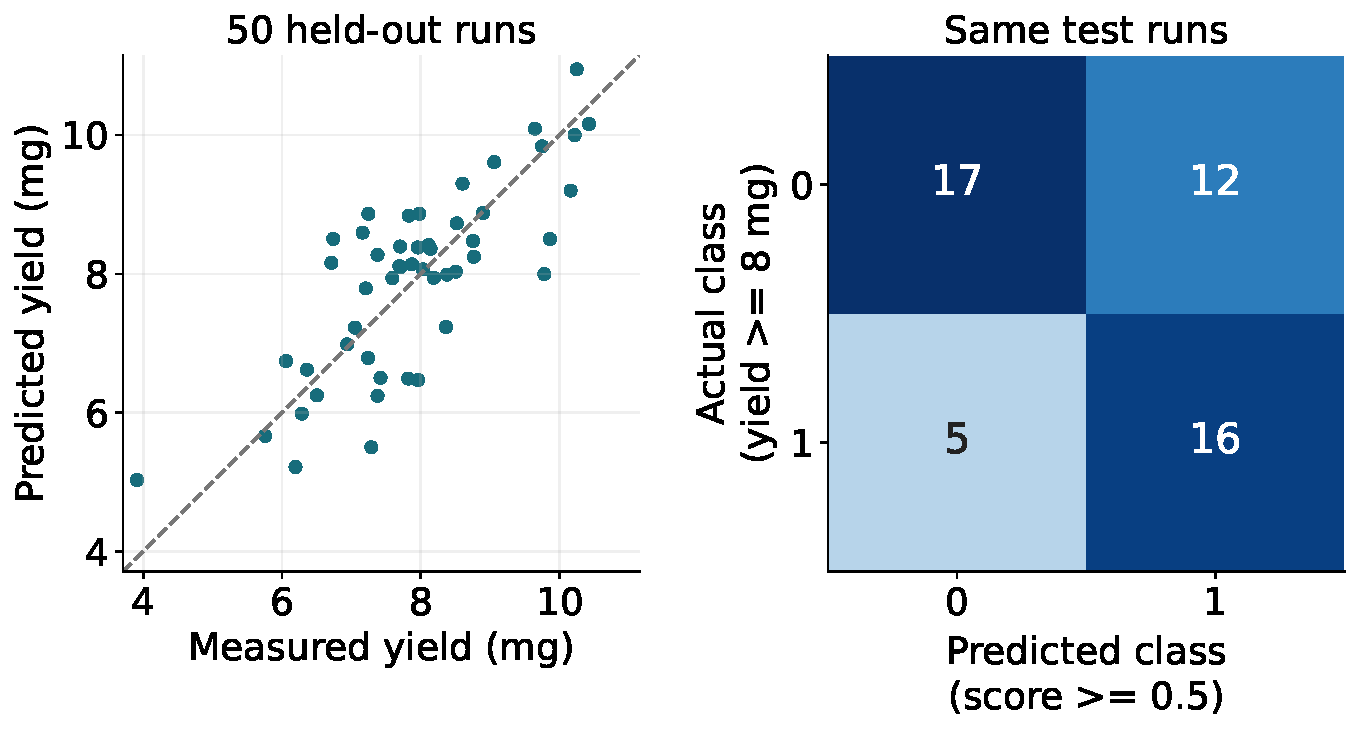
\includegraphics[width=.98\linewidth,height=.69\textheight,keepaspectratio]{heldout-predictions.pdf}\end{frame}
\renewcommand{\notestarget}{notes.pdf\#note-training-only-standardization}
\begin{frame}[t,fragile,label=slide-prediction-on-a-new-experiment]{Prediction on a new experiment}
\begin{verbatim}
X_test_scaled = (X_test - train_mean) / train_scale
prediction = model(X_test_scaled)
\end{verbatim}
\pause{}
Re-estimating the scale from test rows would change the fitted procedure.
\end{frame}
\renewcommand{\notestarget}{notes.pdf\#note-regression-and-classification-errors}
\begin{frame}[t,fragile,label=slide-regression-and-classification-errors]{Regression and classification errors}
\[
\mathrm{RMSE}=\sqrt{\frac1N\sum_i(y_i-\widehat y_i)^2}.
\]
\pause{}
\[
\mathrm{precision}=\frac{TP}{TP+FP},\qquad
\mathrm{recall}=\frac{TP}{TP+FN}.
\]
\end{frame}
\renewcommand{\notestarget}{notes.pdf\#note-regression-and-classification-errors}
\begin{frame}[t,fragile,label=slide-near-boundary-observations]{Near-boundary observations}
An actual yield of $8.1$ mg and a prediction of $7.9$ mg differ by only $0.2$ mg, but fall on opposite sides of the success threshold.
\pause{}
Report the numerical target and decision target separately.
\end{frame}
\renewcommand{\notestarget}{notes.pdf\#note-principal-components}
\begin{frame}[t,fragile,label=slide-principal-components]{Principal components}
\[
\max_{\|v\|_2=1}v^{\mathsf T}X_c^{\mathsf T}X_cv,
\qquad X_c^{\mathsf T}X_cv=\lambda v.
\]
\pause{}
The score of a new row is $s=(x-\mu)v_1$.
\end{frame}
\renewcommand{\notestarget}{notes.pdf\#note-distance-based-groups}
\begin{frame}[label=slide-projection-groups-classification-figure]{Projection groups classification}
\centering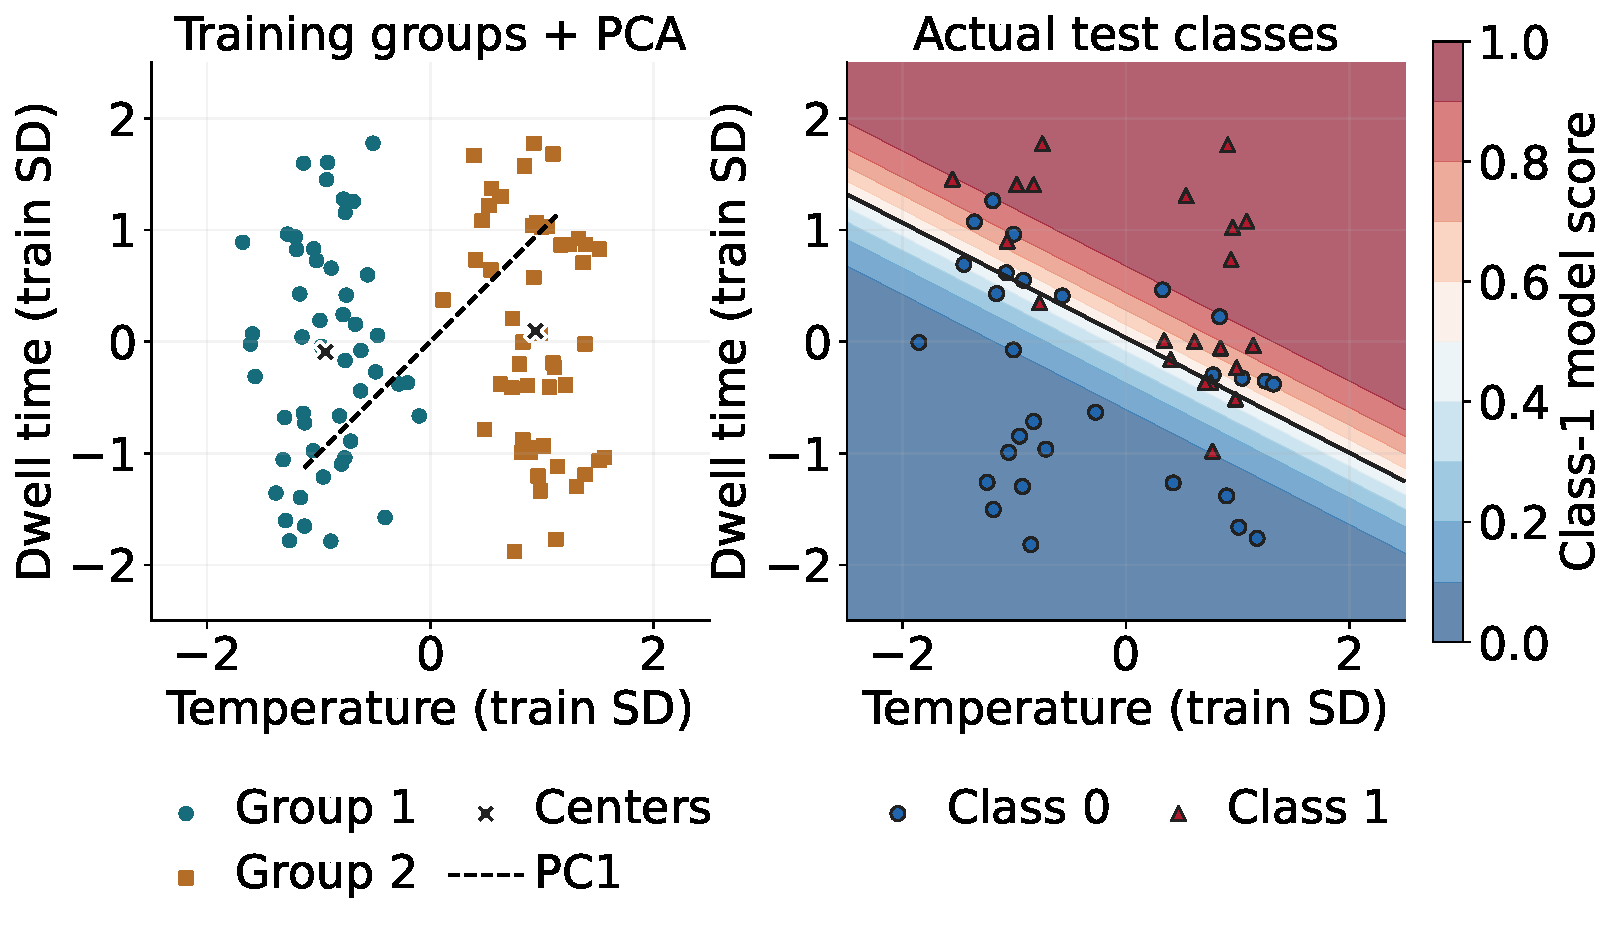
\includegraphics[width=.98\linewidth,height=.69\textheight,keepaspectratio]{presentation-figures/projection-groups-classification.pdf}\end{frame}
\renewcommand{\notestarget}{notes.pdf\#note-principal-components}
\begin{frame}[t,fragile,label=slide-reconstruction-error]{Reconstruction error}
\[
\widehat x=\mu+sv_1^{\mathsf T}.
\]
\pause{}
The lost component $(x-\mu)-sv_1^{\mathsf T}$ is orthogonal to $v_1$. It may still contain information about yield.
\end{frame}
\renewcommand{\notestarget}{notes.pdf\#note-distance-based-groups}
\begin{frame}[t,fragile,label=slide-distance-based-groups]{Distance-based groups}
\[
\min_{\mu_1,\mu_2,c_i}\sum_i\|x_i-\mu_{c_i}\|_2^2.
\]
\pause{}
Cluster assignments depend on predictor geometry, not on the success event.
\end{frame}
\renewcommand{\notestarget}{notes.pdf\#note-regression-and-classification-errors}
\begin{frame}[t,fragile,label=slide-evaluation-after-fitting]{Evaluation after fitting}
Fit scaling, regression, classification, projection and cluster centers using training data.
\pause{}
Evaluate each operation on the held-out experiment using its own stated target. Do not select the best-looking method from repeated test-set inspection.
\end{frame}
\end{document}
